\chapter{Deseño}
\label{chap:deseno}

\section{Análise de requisitos}

A primeira fase foi recoller requisitos e a delineación do dominio do problema a resolver. Para isto realizouse unha reunión inicial cos co-directores do traballo para entender as casuísticas das que nace a necesidade deste traballo. Despois de varias reunións cos co-directores, chegouse aos seguintes casos de uso (véxase diagrama \ref{fig:casosuso}):

\subsection{CU-01: Xestionar modelos}

Da xestión de modelos encárganse os actores Administradores, o que inclúe creación, borrado e modificación.

\subsection{CU-02: Ver modelos}

Ver os modelos inclúese separado de xestionalos, por que é a única acción que pode facer un técnico sobre os modelos; ademais, precísao para poder crear os compoñentes.

\subsection{CU-03: Xestionar compoñentes}

A xestión de compoñentes pode realizarse indistintamente polos actores Técnicos e Administradores, creación, borrado, visualización e modificación.

\subsection{CU-04: Xestionar usuarios}

A xestión de usuarios é exclusiva dos administradores.

\begin{figure}
	\hspace*{-3cm}
	\centering
	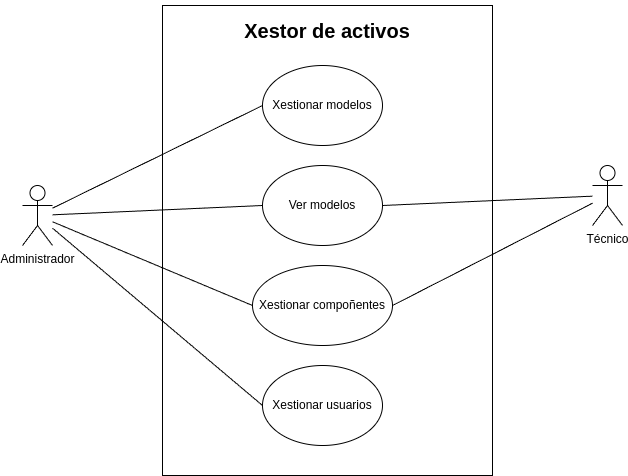
\includegraphics[width=0.7\textwidth]{imaxes/casos_uso.drawio.png}
	\caption{Diagrama de casos de uso}
	\label{fig:casosuso}
\end{figure}

\section{Esquema do sistema}

A plataforma está formada por dous tipos de obxectos: modelos (\Gls{Template}) e compoñentes (\Gls{Component}). Tamén hai dous tipos de usuarios: administradores e técnicos.

\section{Obxectos}

A primeira versión da aplicación presentaba unha serie de obxectos concretos, tales coma servidores ou programas. Porén, tras falar cos codirectores e ver un chisco o uso real por parte de técnicos, escolleuse facer un sistema máis xenérico, que permita adaptarse ás necesidades de cada ambiente. O obxectivo é que cada técnico poida usar a aplicación do xeito que máis se axuste ao seu traballo. A figura \ref{fig:erobxectos} amosa a relación entre os distintos obxectos do sistema.

\subsection{Modelos}

Os modelos representan unha clase de compoñentes. Están formados por campos, e a súa creación correspóndelle aos administradores. Cada campo do modelo deberá indicar se se trata de texto libre, dunha ligazón a unha entidade ou dunha data. As ligazóns deberan apuntar a un compoñente.

\newpage

Dentro da aplicación inclúense algúns modelos predefinidos:

\begin{itemize}
    \item Ordenador
    \item Programa
    \item Licenza
\end{itemize}

Para evitar inconsistencias, non se poden modificar os campos dos modelos se xa teñen compoñentes asociados.

\subsection{Compoñente}

Os compoñentes corresponden a instancias individuais de modelos. Ao crear un compoñente deberanse encher tamén os campos correspondentes. As entidades, segundo se indique no seu modelo correspondente, poden ligarse entre si: ao visualizar unha entidade tamén se poden consultar as entidades que ligan a, e dende, esta.

\section{Usuarios}
\label{sec:usuarios}

\subsection{Administradores}

Os administradores son os usuarios encargados da creación dos modelos para que usen os técnicos. Tamén poderán encargarse da xestión e rexistro de usuarios.

\subsection{Técnicos}

Os técnicos son os usuarios que xestionan os compoñentes, e encárganse de manter actualizada a base de datos durante o transcurso do seu labor.


\begin{figure}
    \centering
    \resizebox{.8\linewidth}{!}{\digraph{"Diagrama esquema-relación"}{
layout=neato;

node [colorscheme = ylgnbu4, shape = none, margin = 0];
edge [colorscheme = dark28, dir = both];

node [shape=box];
	Usuarios;
	Modelos;
	Compoñentes;
	Campos[peripheries=2];
	Datos[peripheries=2];
node [shape=ellipse];
	{node [label="nome"] nome0[label=<<U>nome</U>>]; nome1; nome2[label=<<U>nome</U>>]; nome3[label=<<U>nome</U>>];};
	{node [label="descripción"] descripcion0; descripcion1;};
	contrasinal; rol;
	tipo; contido;
	id[label=<<U>id</U>>];
node [shape=diamond,style=filled,color=lightgrey];
	CD[label="Contén",peripheries=2,color=""];
	MCa[label="Contén",peripheries=2,color=""];
	MC[label="Baseados en"];
	DC[label="Ligazón a"];
	UM[label="Crea e modifica"];
	UC[label="Crea e modifica"];
	CaD[label="Deriva de",peripheries=2,color=""];

Modelos -> MCa [label="1",len=1.25,arrowhead=none,arrowtail=none];
MCa -> Campos [label="n",len=1.50,arrowhead=none,arrowtail=none,color="black:black"];

Modelos -> MC [label="n",len=1.50,arrowhead=none,arrowtail=none];
MC -> Compoñentes [label="1  ",len=1.50,arrowhead=none,arrowtail=none,color="black:black"];

Compoñentes -> CD [label="1  ",len=1.50,arrowhead=none,arrowtail=none];
CD -> Datos [label="n",len=1.50,arrowhead=none,arrowtail=none,color="black:black"];

Datos -> DC [label="n",len=2.00,arrowhead=none,arrowtail=none];
DC -> Compoñentes [label="m",len=2.00,arrowhead=none,arrowtail=none];

Campos -> CaD [label="1     ",arrowhead=none,arrowtail=none];
CaD -> Datos [label="n",arrowhead=none,arrowtail=none,color="black:black"];

Usuarios -> UM [label="n",len=1.50,arrowhead=none,arrowtail=none];
UM -> Modelos [label="m",len=1.50,arrowhead=none,arrowtail=none,color="black:black"];
Usuarios -> UC [label="n",len=1.50,arrowhead=none,arrowtail=none];
UC -> Compoñentes [label="m",len=1.50,arrowhead=none,arrowtail=none,color="black:black"];

nome0 -> Usuarios[arrowhead=none,arrowtail=none];
nome1 -> Compoñentes[arrowhead=none,arrowtail=none];
nome2 -> Modelos[arrowhead=none,arrowtail=none];
nome3 -> Campos[arrowhead=none,arrowtail=none];

descripcion0 -> Modelos[arrowhead=none,arrowtail=none];
descripcion1 -> Compoñentes[arrowhead=none,arrowtail=none];

id -> Compoñentes[arrowhead=none,arrowtail=none];

contrasinal -> Usuarios[arrowhead=none,arrowtail=none];
rol -> Usuarios[arrowhead=none,arrowtail=none];

tipo -> Campos[arrowhead=none,arrowtail=none];
contido -> Datos[arrowhead=none,arrowtail=none];
}}
    \caption{Diagrama Esquema-Relación dos obxectos do sistema}
    \label{fig:erobxectos}
\end{figure}

\section{Busca}

A busca realízase mediante unha serie de comparacións entre propiedades e valores, unidas mediante operacións lóxicas.

As propiedades serán da forma «\textit{obxecto}.\textit{atributo}». Os obxectos serán os indicados na sección anterior. Os atributos poderán ser calquera dos indicados na figura \ref{fig:erobxectos}. Poderán compararse os contidos e atributos dos campos de compoñentes e modelos usando a mesma sintaxe de atributos separados por puntos. A propiedade que representa o valor dos campos é especial, e, dependendo da operación, só coincidirá con certos tipos de campos.

Para detalles máis específicos, véxase a sección \ref{sec:busca}.

Existen tres grupos de operacións a realizar: sobre cadeas, sobre números e sobre conxuntos.

As operacións sobre cadeas realizan unha comparación usando expresións regulares Para a comparación úsanse os operadores \textasciitilde e !\textasciitilde para a versión negada. A operación sobre cadeas pódese usar sobre todas as propiedades; se se aplica sobre o valor dos campos só coincidirá en campos de tipo texto ou data (neste caso sobre a representación textual da data). Esta operación pode usarse sobre todas as propiedades, e no caso do valor dos campos sobre os de tipo cadea e data (neste caso sobre a representación textual das mesmas).

As operacións sobre conxuntos son equivalentes a realizar unha serie de operacións sobre cadeas, unidas por disxuncións lóxicas. Úsanse coma operadores «@» ou «!@» (versión negada), e seguido unha listaxe de cadeas entre corchetes separadas por comas. Deste xeito, \texttt{template.name @ [ "A", "B", "C" ]} é equivalente a facer \texttt{template.name \textasciitilde "A" | template.name \textasciitilde "B" | template.name \textasciitilde "C"} Esta operación pode usarse sobre as mesmas propiedades ca as sobre cadeas, e tamén nos valores dos campos de tipo numérico e ligazóns, que deberán ser números completos e non expresións regulares.

As operacións sobre números aplícanse exclusivamente ao valor de campos, e só aos de tipo número, data e ligazón. As condicións posibles serán de maior (ou igual) que, menor (ou igual) que, igual ou non igual. Nas datas compararase se o valor é posterior ou anterior á data indicada. Para as ligazóns só se poderán usar as condicións de igualdade ou non igualdade.

\newpage

As operacións lóxicas son a conxunción (co operador «\&») e a disxunción (co operador «|»). Ambas operacións teñen a mesma precedencia e asócianse de esquerda a dereita, de xeito que \texttt{a | b \& c} é o mesmo que \texttt{ (a|b) \& c }. Pódense usar parénteses para indicar a precedencia.

Isto da coma resultado a seguinte gramática independente do contexto en forma Backus–Naur:

\begin{grammar}
	<expresión> ::= <proba>
	\alt '(' <expresión> ')'
	\alt <expresión> '\&' <expresión>
	\alt <expresión> '|' <expresión>
	
	<proba> ::= <propiedade> ( `~' | `!~' ) <cadea>
	\alt <propiedade> ( `>=' | `<=' | `>' | `<' | `=' | `!=' ) ( <número> | <data> )
	\alt <propiedade> ( `@' | `!@' ) `[' <cadea> (',' <cadea>)* `]'
\end{grammar}

Os elementos terminais defínense usando expresións regulares. \texttt{<número>} defínese coma un número racional ([+-]?[0-9]+\allowbreak{}(\.[0-9]+)?), \texttt{<cadea>} defínese coma calquera número de caracteres entre comiñas sen escapar (\verb|[^\]".*[^\]"|) e \texttt{<data>} defínese usando o formato ISO 8601\footnote{UNE-EN 28601:1995 na normativa española\cite{iso8601}} para data e hora sen incluír fuso horario ([0-9][0-9][0-9][0-9]-\allowbreak{}[0-9][0-9]-\allowbreak{}[0-9][0-9]T\allowbreak{}[0-9][0-9]:\allowbreak{}[0-9][0-9]:\allowbreak{}[0-9][0-9]).

Para a interpretación defínense dúas gramáticas: unha para a análise léxica e a outra para a análise sintáctica.

Na análise léxica defínese un alfabeto que inclúe todos os caracteres Unicode, limitado únicamente polos caracteres que acepta Java e PostgreSQL para cadeas. Sobre este alfabeto defínense certas linguaxes regulares: as xa indicadas previamente para definir números racionais, datas e cadeas; xunto coas que aceptan os operadores, comas, parénteses e corchetes.\footnote{Non se definen estas últimas pola súa simplicidade}. A definición da gramática que acepta propiedades sería

\begin{eqnarray}
l \in \{ a,b,c,d,e,f,g,i,j,k,l,m,n,ñ,o,p,q,r,s,t,u,v,w,x,y,z \} \\
p = l^{\ast}(.l^{\ast})^{\ast} 
\end{eqnarray}

\newpage

Na análise sintáctica defínese un alfabeto baseado no resultado da análise léxica:

\begin{equation}
\begin{gathered}
\Sigma = \{ \text{propiedade}, \text{comparación}, \text{non comparación}, \\
	\text{maior que}, \text{menor que}, \text{maior ou igual que}, \\
	\text{menor ou igual que}, \text{igual que}, \text{non igual que}, \\
	\text{en conxunto}, \text{non no conxunto}, \text{paréntese aberto}, \\
	\text{paréntese pechado}, \text{corchete aberto}, \text{coma} \\
	\text{corchete pechado}, \text{cadea}, \text{número}, \text{data}, \text{conxunción}, \text{disxunción} \}
\end{gathered}
\end{equation}

Entre o paso léxico e sintáctico elimináronse os espazos en branco, saltos de liña ou calquera outros caracteres que non afectan á sintaxe, execepto dentro de cadeas.

Como nesta gramática existen producións con varias expresións non terminais, precísase pasar dunha gramática regular a unha independente do contexto, e deste xeito poder usar operacións de conxunción e disxunción dunha forma moito máis lexible. Se non, habería que usar algunha notación prefixo ou limitar moito que tipo de comparacións poderíanse facer.\cite{teoria_automatas}

A modo de exemplo, vaise converter a cadea «\textit{(user.name @ ["root", " 12 "] \& user.role !@ [ "NORMAL" ]) | template.name \textasciitilde "y" \& template.name @ [ "A" ] \& component.field.value > 2}». Primeiro divídese mediante análise léxica, ignorando os espazos en branco:

\begin{eqnarray}
\underset{\text{paréntese aberto}}{(} \underset{\text{propiedade}}{user.name} \underset{\text{en conxunto}}{@} \underset{\text{corchete aberto}}{[} \underset{\text{cadea}}{"root"} \underset{\text{coma}}{,} \underset{\text{cadea}}{" 12 "} \underset{\text{corchete pechado}}{]} \underset{\text{conxunción}}{\&} \\
\underset{\text{propiedade}}{user.role}\underset{\text{non no conxunto}}{!@} \underset{\text{corchete aberto}}{[} \underset{\text{cadea}}{"NORMAL"} \underset{\text{corchete pechado}}{]} \underset{\text{paréntese pechado}}{)} \underset{\text{disxunción}}{|} \underset{\text{propiedade}}{template.name} \\
\underset{\text{comparación}}{\textasciitilde} \underset{\text{cadea}}{"y"} \ldots
\end{eqnarray}

A partir disto xerase a árbore de sintaxe (figura \ref{fig:arboresintaxe}):

\begin{figure}[H]
	\centering
	\resizebox{.8\linewidth}{!}{\begin{tikzpicture}
\Tree [.expresión(disxunción)
	[.expresión(parénteses)
		[.expresión(disxunción)
			proba(listas)
			proba(listas)
		]
	]
	[.expresión(conxunción)
		proba(cadeas)
		[.expresión(conxunción)
			proba(listas)
			proba(números)
		]
	]
]
\end{tikzpicture}}
	\caption{Árbore de sintaxe de exemplo}
	\label{fig:arboresintaxe}
\end{figure}